\chapter{Thesis Background}
\label{sec:backgroundthesis}

This chapter is about the background of the thesis, in order to understand better further chapters and as a help and reference to reproduce the results of this thesis in the future. 

\section{PYNQ-Z2 Development Board}
The \textit{PYNQ-Z2} is a development board designed for the Xilinx University Program. It is equipped with a Xilinx ZYNQ 7020 SoC (XC7Z020-1CLG400C), 512 MB of DDR3 RAM and 16 MB of QSPI Flash Storage. The board provides a clock reference thanks to a crystal oscillator with a frequency of 50 MHz. The reference clock is used by the PS and can be provided to the PL too. 

\begin{figure}[H]
\centering
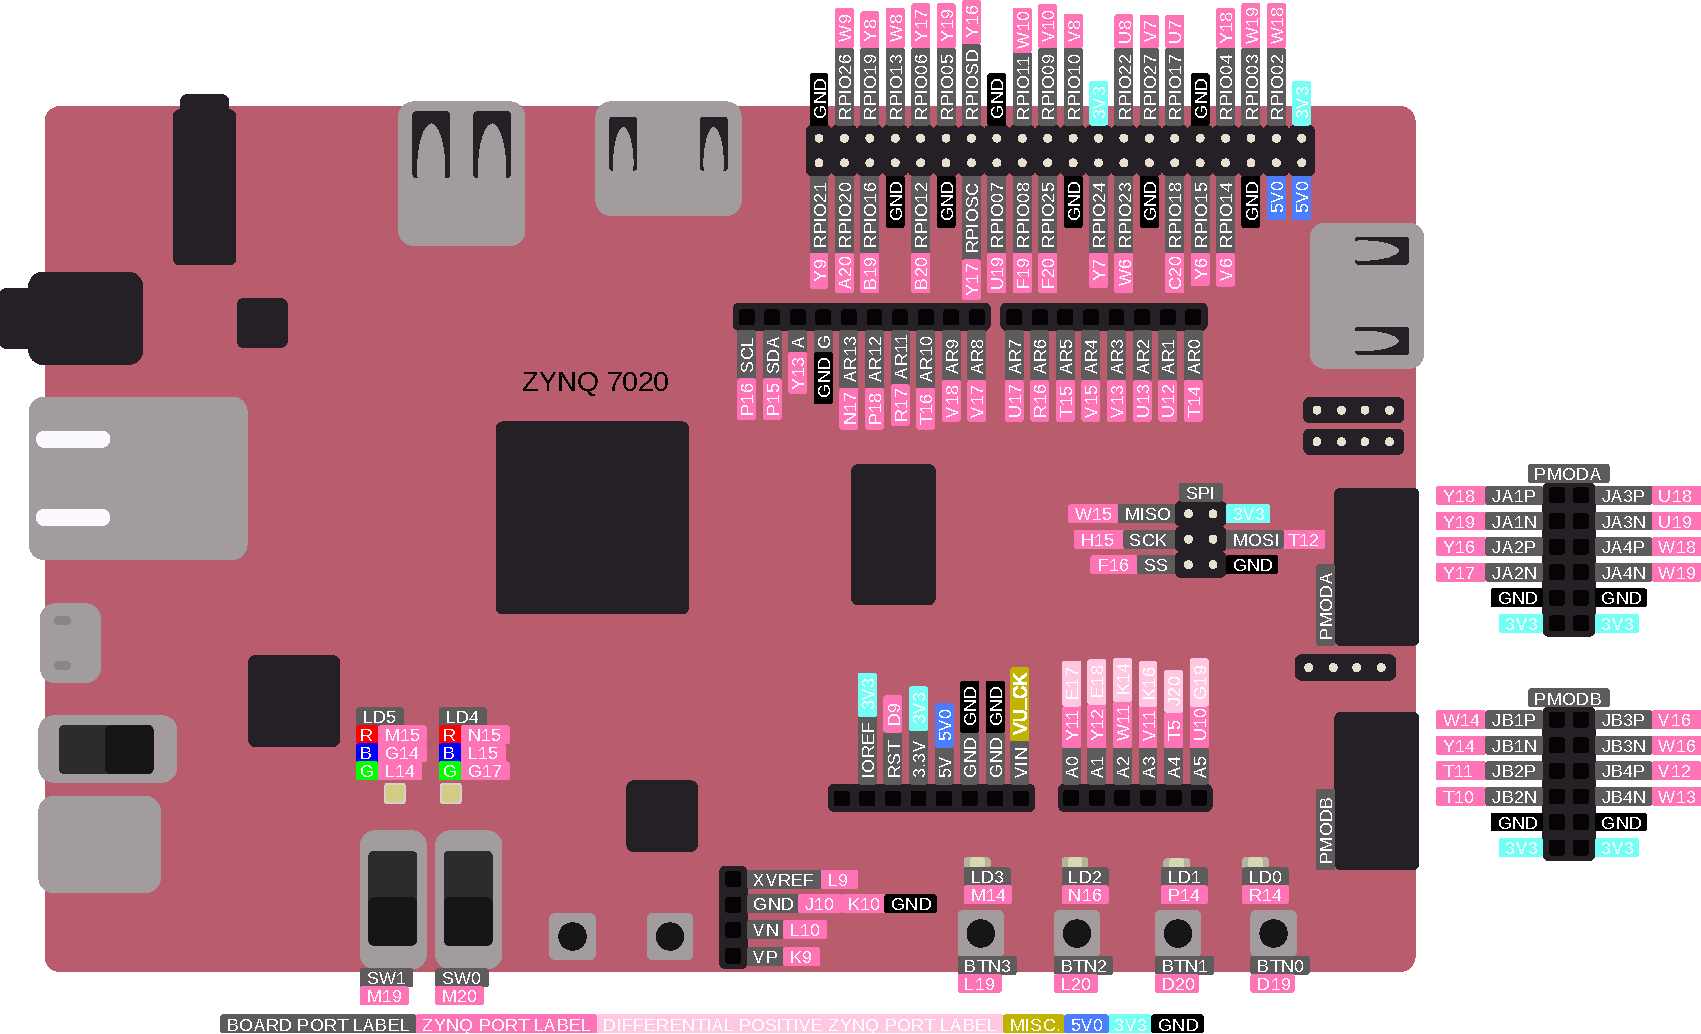
\includegraphics[width=0.7\linewidth]{images/chapter3/PINOUT.pdf}
\caption{Schematic of the PYNQ-Z2 Development Board}
\label{fig:pynqz2}
\end{figure}

The SoC is made of two subparts: a Processing System (PS) and a Programmable Logic (PL). The PS is the main part of the SoC, containing two 650 MHz ARM Cortex-A9 processor, 512 KB L2 Cache, 256 KB On-Chip Memory and other modules like FPUs, Flash Controller, DRAM Controller, GPIOs and so on.

\begin{figure}[H]
\centering
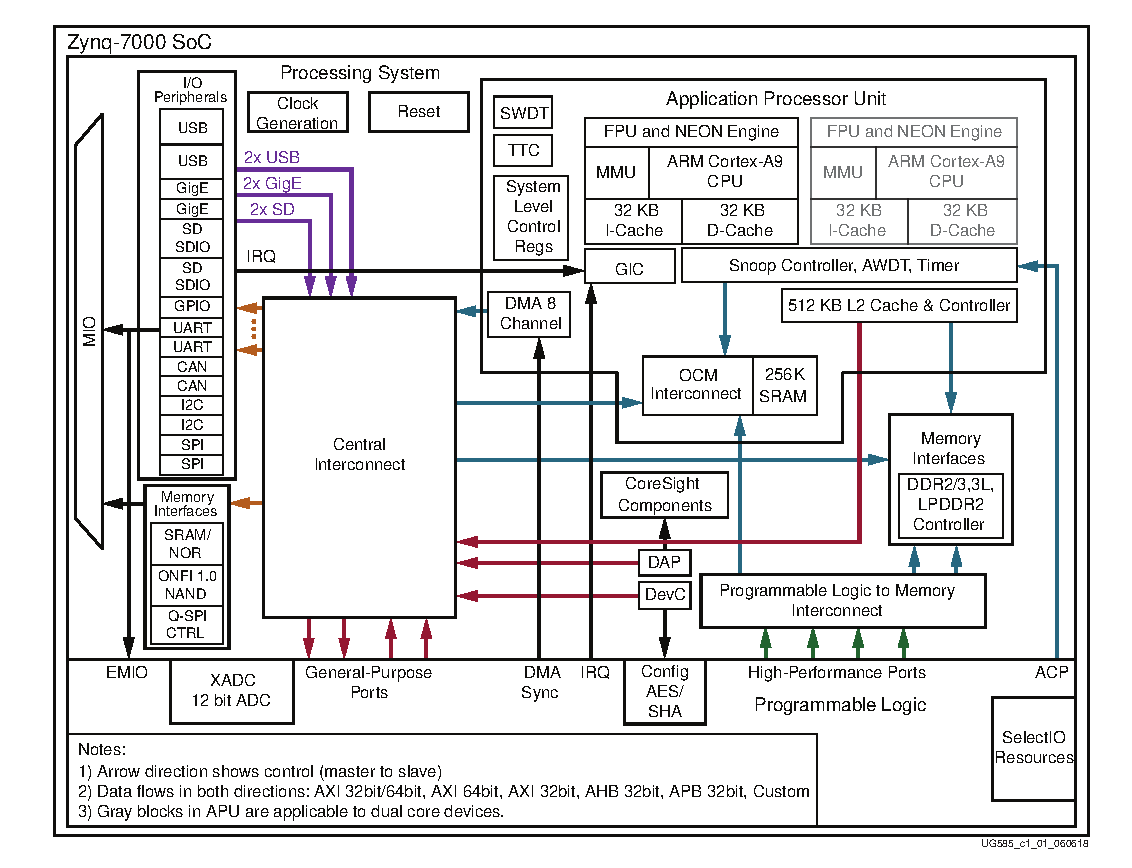
\includegraphics[width=1.0\linewidth]{images/chapter3/zynq.pdf}
\caption{Schematic of ZYNQ 7020 SoC}
\label{fig:zynq7020}
\end{figure}

A schematic is shown in Figure \ref{fig:zynq7020}. The second part is the PL, which consists in a FPGA with the following characteristics:

\begin{itemize}
    \item 13,300 logic slices, each with four 6-input LUTs and 8 flipflops
    \item 630 KB block RAM
    \item 220 DSP slices
    \item On-chip Xilinx analog-to-digital converter (XADC)
\end{itemize}

The PL can access the Processing System's memory space through a High Performance and/or General Purpose AXI Ports. This enables the usage, for example, of the DDR3 RAM and of the On-Chip memory (OCM) from the PL. The board can be programmed through a JTAG interface, which allows to upload a firmware to be executed from the PS or to program the PL via a bitstream. Moreover, it provides a virtual UART interface that can be used as input/output both for the PS and the PL.\bigskip

\begin{bytefield}{24}
    \memsection{0xbfff\_ffff}{0x4000\_0000}{3}{PL}\\
    \memsection{0x3fff\_ffff}{0x0000\_0000}{3}{OCM/DDR}
\end{bytefield}

% \subsection{Configuration Ports}

\section{Xilinx's Microblaze soft-core}




\section{Xilinx FPGA Standard Design Flow}
\subsection{Bitstream Generation}
\subsection{Fundamentals of the Xilinx's Bitstream structure}
\subsection{Software Development}
% talk about Vitis and xsct
\section{Fault Injection Tool}